\fancychapter{Related Work}\label{chap:related}
\cleardoublepage{}

\section{Fault Models}\label{sec:related_fault_models}

In this section, we survey the most used classes of fault models
for distributed systems and compare them the novel
\ac{RR} model. It is important to first clarify that, both
here and in the rest of this document, we consider the network to
be asynchronous. This means that the upper bound for the message
delivery delay between replicas is unknown, and may not even
exist. This model is consistent with the Internet, where network
partitions may temporarily impede or arbitrarily slow down the
communication between two nodes.

\paragraph{Crash fault models.} A crash fault is said to have
occurred when a node stops replying to requests. This may happen
for several reasons: power outages, network
partitions, programming errors that
cause the processes to crash, etc. A crash fault can be
considered \emph{fail-stop} if other processes can detect that it
has in fact crashed. However, perfect failure detection in asynchronous
systems is impossible~\cite{perfect-failure-impossible}. A node that
suffers a crash fault is indistinguishable from an extremely slow
one~\cite{polynomial-communication} (rigourously, a node which replies at $t = \infty$).  The
\emph{crash-recovery}
model~\cite{consensus-recovery,crash-recovery} is a slight variation from the crash
model, wherein replicas are allowed to restart and run a recovery
protocol.

\paragraph{Byzantine fault models.}
First introduced by Lamport et al in~\cite{lamport:byzgenerals},
a Byzantine fault is the most encompassing type of fault
possible, since it assumes nodes can deviate arbitrarily from the
prescribed protocol. They may do so maliciously or simply by component
or programming error. Furthermore, several Byzantine nodes may
collude to deviate in a coordinated fashion, in an attempt to
subvert the guarantees of the system. Compared to crash fault
tolerant protocols, \ac{BFT} protocols are expensive on account of
mechanisms such as digital signatures~\cite{bqs} or extra protocol
rounds~\cite{pbft}.

\paragraph{Hybrid fault models.}
Hybrid fault models consider at least two types of faults
separately. They have the advantage of better adapting the
system parameterization to the deployment conditions by offering
greater flexibility, at the cost of some complexity.
UpRight~\cite{upright} is an example of a system which uses such
a hybrid fault model, concretely a hybrid crash-\ac{BFT} model, where
the system is able to sustain a different number of crash and
Byzantine faults. In particular, UpRight sustains $u$ crash faults in addition
to $r$ commission faults, which are a subset of Byzantine faults
where nodes actively produce an incorrect message (and thus
excluding the subset of crash faults from the Byzantine failure
model). This leads to an elegant reasoning about Byzantine fault
tolerance that separates incorrect from non-incorrect node
behavior.

Besides protocol changes, different fault models require
different quorum systems. A \emph{quorum} is defined as the
minimum set of replies that need to be gathered to proceed to the
next step of the protocol. The size of quorums is of great
importance for the economical cost of systems, as larger quorums require
more replicas and resources, as well as their performance, as
larger quorums will generally take longer to gather. These
quorums not only depend on the fault model, but on the network
model and synchrony assumptions. As an example,
Table~\ref{tab:quorum} has the quorum sizes for the crash,
Byzantine and UpRight models in the asynchronous model.

\begin{table}[ht]
    \centering
    \caption{Quorum sizes in different fault models. In the crash
    model $f$ is the number of crashed replicas, in the Byzantine
    model $f$ is the number of Byzantine replicas, and in the
    UpRight model $u$ is the number of crash faults and $r$
    the number of commission faults tolerated.}
    \begin{tabular}{|l|c|c|c|}
        \hline
        \textbf{Fault Model} & \textbf{Fault Parameter} & \textbf{\# Replicas} & \textbf{Quorum Size} \\
        \hline
        Crash & f & 2 f + 1 & f + 1 \\
        \hline
        Byzantine & f & 3 f + 1 & 2 f + 1 \\
        \hline
        UpRight & u, r & 2 u + r + 1 & u + r + 1 \\
        \hline
    \end{tabular}\label{tab:quorum}
\end{table}

\paragraph{Comparison to \ac{RR}.}
The \ac{RR} model allows for the system to tolerate a combination of
crash faults and faults where a replica has stale state after a
restart. The \ac{RR} model is strictly more encompassing than
the crash model, allowing for fault behaviors that are
not tolerated by this. Compared to \ac{BFT}, it does not need to
protect against generic Byzantine faults, leading to simpler,
more efficient protocols with smaller quorums in the common case.
Finally, compared to hybrid crash-\ac{BFT}
models~\cite{MeyerPradhan91,bc:hybrid,mc:hybrid,upright}, while
\ac{RR} is also a hybrid model, it differs in the type of
non-crash behavior it admits, since wrong answers in \ac{RR}
are limited to rollbacks after a restart, whereas previous hybrid
models tolerated arbitrary Byzantine faults.

The \ac{RR} model has some relevant characteristics such as
leading to dynamic quorum sizes, where the size depends on the
number of replies from recently restarted nodes, leading to small
read quorums in the normal case. Other proposals, such as Refined
Quorum Systems~\cite{rqs} or Flexible Paxos~\cite{fp},  also use
varying quorum sizes in different parts of the protocol. However,
they do it in a way that is complementary to ours, since they
work on traditional models (crash and Byzantine) and come up with
protocol techniques based on different quorum sizes to improve
performance. In contrast, \ac{RR} is a new model (based on a
different set of assumptions) that naturally leads to dynamic
quorums.

Another approach of hybrid quorums has been put forward by
\ac{VFT}~\cite{visigoth}. In \ac{VFT} not only are crash and
commission faults separately considered, the synchrony of the
system is also a parameter of the quorum system. This allows
\ac{VFT} to be parameterized as either synchronous or asynchronous
and as either crash or Byzantine, with hybrid combinations.
Although an interesting contribution, we consider \ac{VFT} to be
an orthogonal approach.

\section{Replication Protocols}
Replication is a technique wherein multiple copies of a service run
simultaneously so that the overall system maintains its operation
even in the presence of faults. There are several protocols for
replicated services, varying vastly according to the types of
faults tolerated, performance characteristics and semantics of
the service. In this section, we will survey two types of
services frequently replicated: read-write registers and state
machines.

\paragraph{Read-Write Register.} A read-write register supports a
very simple interface, allowing clients to either read the
current value or writing a new one. Due to their simplicity,
protocols for replicating registers are considered to be quite
fast. The ABD protocol proposed by Attiya
\emph{et al.}~\cite{abd} implements this register in the crash
model, while the Malkhi and Reiter proposed a Byzantine fault tolerant
counterpart in~\cite{bqs}.

\paragraph{State Machine Replication.} A deterministic state machine (SM) is a
mathematical construct that supports the successive application of
\emph{operations}, which mutate its internal state. This is a
powerful programming abstraction, as it can simulate any
deterministic computation. For that reason, it has been the
object of much research within the distributed systems community:
using state machine replication (SMR), system builders can build
arbitrarily complex fault tolerant systems~\cite{schneider-smr} (provided that they
are deterministic). A common method for achieving SMR is to
attach a \emph{consensus} module to an operation log. Consensus
is a process by which a set of nodes agree on a value. By agreeing
on the value for each entry in the log, replicas can then be sure
that they apply the same operations to their local state machines in the same order,
guaranteeing that their state is consistent. Importantly,
Fischer, Lynch and Paterson proved that consensus is impossible
in a fully asynchronous network~\cite{flp}. As a result,
consensus protocols make synchrony assumptions in certain places.

The Paxos protocol~\cite{paxos} proposed by Leslie Lamport, which
is applicable to the crash model, has been widely studied, with
multiple variants being
proposed~\cite{fp,fast-paxos,egalitarian-paxos,disk-paxos,paxos_builders}.
Raft~\cite{raft} is an alternative protocol for SMR in the crash
model, developed with the goal of being easy to understand and
implement. The PBFT~\cite{pbft} protocol developed by Castro and
Liskov provides SMR in the Byzantine model.

\section{Trusted Execution Environments}
Recent generations of general-purpose CPUs, namely the ones that
support Intel SGX~\cite{intelsgx}, Intel TDX~\cite{inteltdx}, AMD
SEV-SNP~\cite{amdsev,amdsev-snp}, or ARM TrustZone~\cite{armTZ}
technology, include support for trusted execution environments (TEEs),
allowing users to deploy a computation with hardware-enforced
confidentiality and integrity on a compute platform that is not under
their control.  TEEs have been used to protect the integrity and
confidentiality of generic applications running on commodity operating
systems~\cite{haven}, as well as of large-scale distributed
computations~\cite{vc3}. Microsoft and Google both offer VMs with TEE
support as part of their Cloud
services~\cite{azure-conf,google-confVM}.

\paragraph{Built-in storage support for TEEs.}
Current TEEs offer some support for securely storing persistent
data in an encrypted form outside the TEE, such that it can be
decrypted only by the TEE that stored it if and only if it was not
modified. If this support would offer perfect protection, then a
CFT replication protocol might suffice to replicate TEE-based
systems. However, different systems have different limitations
that preclude a direct use of CFT.  In particular, ARM
TrustZone-based devices include an eMMC storage controller that
allows for configuring a small storage partition (on the order of
tens of megabytes), named the ``Replay Protected Memory Block''
(RPMB), which only accepts commands from authenticated secure
world domains, and withstands rollback attacks~\cite{rpmb}.
However, the size and access to this block is quite inflexible:
the RPMB is configured as a separate partition of the eMMC
storage device, and a shared cryptographic secret must be
embedded in the host and the storage device during manufacture.
Intel SGX supports data sealing, i.e., encrypting it in a way
that it can be decrypted only by the same enclave on the same
platform~\cite{intelsgx}. However, this abstraction alone does
not protect against rollback attacks, where an attacker replaces
the most recent sealed data object stored in an untrusted medium
with a stale version of the object~\cite{memoir}. Recent versions
of SGX use a persistent, monotonic counter that is uniquely tied
to the TEE instance by packaging the counter storage physically
with a CPU, which is itself tied to the TEE~\cite{intelsgx}. Upon
sealing, this counter is read from the CPU, incremented and
stored with the sealed data. Upon unsealing, the counter that was
previously stored with the data is compared to the current
counter value in the CPU. However, the authors of a recent
paper~\cite{rote} note that writes to the Intel SGX monotonic
counter are very slow (on the order of hundreds of milliseconds)
and that wear can cause its memory to fail after a few days of
continuous use.

\paragraph{Protection against rollback attacks.}
The storage associated with the TEE can also be secured using
methods other than the built-in support. The strategies used by
these methods fall into two categories. The first category of
defenses relies on a small amount of non-volatile state tied to
the TEE platform, which is used to assert the freshness of the
TEE's externally stored state upon a restart of the TEE.
Memoir~\cite{memoir} relies on a TPM~\cite{tpm} to store a hash
chain of all external state updates.  To avoid wearing out the
TPM's NVRAM, whenever the TEE executes an operation, it extends
the hash chain in a volatile TPM PCR register. Upon power
failure, an uninterruptible power supply is used to run a
shutdown handler that copies the latest PCR value into the TPM's
NVRAM.  ICE~\cite{ice} relies on a specialized CPU extension with
volatile ``guarded memory'', which stores the latest freshness
information. During a power failure, a capacitor supplies enough
power for the CPU to write the freshness information into
off-chip, untrusted NVRAM. Ariadne~\cite{ariadne} writes
freshness information to on-chip NVRAM, but minimizes wear by
using a Gray code to represent a monotonic counter, such that any
increment requires only a single bit flip. Ariadne also describes
an attack with the ``store-then-increment'' monotonic counter
approach where a TEE is made to crash repeatedly between the
store and the counter increment, and proposes a fix by
incrementing the counter twice upon a recovery from a crash.

The drawback of defenses in this category is that, in practice,
either the rate at which a TEE can save its state is limited by
wear of the non-volatile memory (latest SGX, Ariadne), or there
is a dependency on specialized hardware or an uninterruptible
power supply (ICE, Memoir). A second category of defenses stores freshness information in a
separate trusted server, or set of servers that are assumed to
not all be subject to a coordinated rollback attack.

An approach called ROTE~\cite{rote} addresses the performance and
wear shortcomings of monotonic counters in Intel SGX by
replicating a monotonic counter in several TEEs, using what is a
hybrid crash-BFT protocol~\cite{MeyerPradhan91, upright}, where a
subset of the replicas may become unavailable and another subset
may return arbitrary results. However, since ROTE maintains the
counter in the enclave's volatile memory, it will lose the
counter state after a simultaneous restart of all replicas, e.g.,
due to a system-wide power failure. Moreover, the use of BFT is
too pessimistic and leads to costly replication and poor
performance, as we discussed.

Defenses in both categories, although adequate for single-client
applications, fundamentally cannot support concurrent sharing
between clients since they do not provide atomic updates of data
and metadata.

\paragraph{Protection against forking attacks.}
A forking attack on a TEE occurs when two instances of the same
enclave are created and executed in parallel, unbeknownst to each
other. Such an attack can create a branch in the state of the
TEE, breaking state continuity. To circumvent these issues, there
are three main approaches, either relying on trusted monotonic
counters~\cite{rote,ariadne,a2m,trinc,memoir},  on client
cooperation/intervention~\cite{fork_verify,fork_fail,fork_comm,fork_lcm,fork_sporc,fork_fs,fork_venus}
or  on some centralized (possibly replicated) source of
truth~\cite{haven}. Relying on monotonic counters shares the
disadvantages already discussed, and relying on clients may be
impractical or even impossible (as it requires mutual trust
between clients or they being online). In the context of
replicated systems, using the system configuration (modified
using consensus) as the source of truth is a natural mechanism to
prevent forking attacks.

\paragraph{Replication using \acp{TEE}.}
There are some proposals that, although not focusing specifically
on the problem of persistence, share the goal of improving replication
protocols through trusted components. These can be broadly divided into
proposals that run an entire replica inside a trusted
component~\cite{p2p-sgx,bft-sgx} and those that augment the replica logic with a
small trusted module~\cite{a2m,trinc}.  However, their technical solutions are
inherently different from the ones we adopt, because they either
trust the entire replica or have a trusted computing base that is
constrained by the hardware (e.g., a trusted monotonic counter).
In contrast, our work focuses on a setting where the computation is
trusted but the persistent storage is not.

\section{Single-node \acfp{KVS}}

One way of implementing replicated \acp{KVS} is to implement a
replication layer on top of a single-node \ac{KVS}. Consequently,
it is important to understand the overall design of a single-node
\ac{KVS}, as well as its tradeoffs.

\subsection{\acfp{LSM-tree}}

\begin{figure}[t]
    \centering
    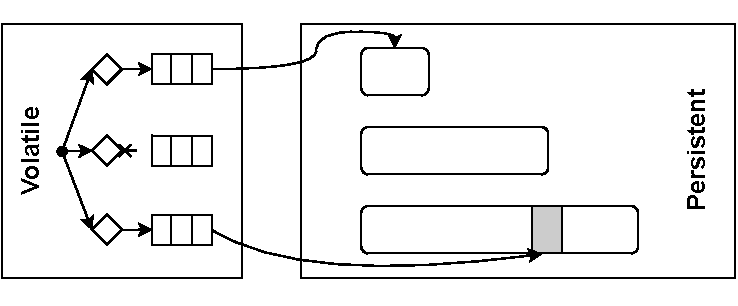
\includegraphics[width=\linewidth]{img/lsm_read}
    \caption{\acf{LSM-tree}. A read request first consults the
    bloom filters (in this case, the first yields a false
    positive, the second a true negative and the third a true
    positive) and subsequently performs a binary search on the
    fence pointers to find the block to get in each run, finding
    the target key (shaded) in the third
    run.}\label{fig:lsm_read}
\end{figure}

The key data structure for modern \acp{KVS} is the \acf{LSM-tree}.
Examples of industry-grade \acp{KVS} relying on \acp{LSM-tree} include
LevelDB~\cite{leveldb},
BigTable~\cite{bigtable}, Apache Cassandra~\cite{cassandra} and
RocksDB~\cite{rocksdb}. \acp{LSM-tree} have also been the topic of
a lot of recent research~\cite{lsm1,lsm2,lsm3,lsm4}.


The main objective of \acp{LSM-tree} is to improve the
scalability of both reads and writes of persistent \acp{KVS}. To
scale writes, the \ac{LSM-tree} creates an in-memory batch of
objects. Once it has filled up, it sorts the batch and sends it
to disk where it becomes a \emph{run}. To keep the data organized
for efficient reads, the \ac{LSM-tree} maintains similarly sized
runs on levels of exponentially increasing sorted runs. Once a
particular level becomes too full, it is sort-merged into a run
of the following level. To perform a read, a binary search is
performed on each run to find the object. To optimize IO costs,
two approaches are employed. First, arrays of fence pointers are
stored in memory, which allows us to perform the binary searches
in memory, reducing the IO cost per run to 1. Additionally, a
Bloom filter~\cite{bloom} can be constructed per run to filter
upfront which runs need not be checked. Figure~\ref{fig:lsm_read}
summarizes the architecture of an \ac{LSM-tree} responding to a
read request.


\begin{figure}[t]
    \begin{minipage}[t]{0.45\linewidth}
        \centering
        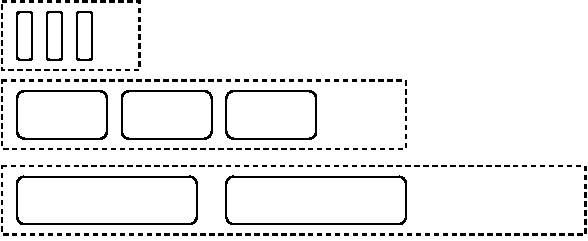
\includegraphics[width=\linewidth]{img/lsm_tiered}
        \caption{Tiered \ac{LSM-tree}.}\label{fig:lsm_tiered}
    \end{minipage}
    \begin{minipage}[t]{0.45\linewidth}
        \centering
        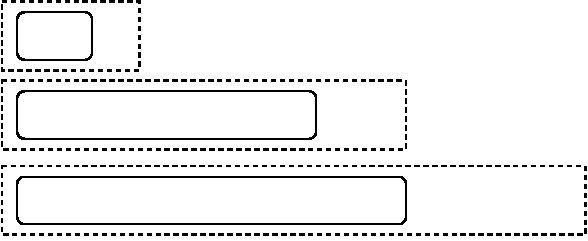
\includegraphics[width=\linewidth]{img/lsm_leveled}
        \caption{Leveled \ac{LSM-tree}.}\label{fig:lsm_leveled}
    \end{minipage}
    \caption{Comparison between a tiered and leveled
    \ac{LSM-tree}. The dashed boxes represent the capacity of the
    level and contiguous blocks denote sorted runs. In the tiered
    \ac{LSM-tree}, adding another run to the first level would
    trigger a sort-merge which would create another run at the
    second level. In the leveled \ac{LSM-tree}, each level is already sorted. }
\end{figure}

There are two classes of designs for \acp{LSM-tree}, levelling
and tiering \acp{LSM-tree}. In the tiereing approach, each level
gathers runs from the previous level, sorting them only when it
reaches capacity and pushing the newly-sorted run to the next
level. In the levelling approach, a run from the previous level
is merged as soon as it is received, ensuring the run is always
sorted. The tiering approach is tailored to write-intensive
workloads, since it does less work per object, while the
levelling approach is more read-optimized, as the runs are in a
sorted state, allowing for more efficient lookups.
Figures~\ref{fig:lsm_tiered} and~\ref{fig:lsm_leveled} show the
two different approaches.


\section{Persistence in replicated distributed systems}

The means by which persistence is achieved in replicated
systems is non-consensual within the distributed systems
community. Some authors consider that persistence requires
synchronizing the state of the replicas to a persistence
medium~\cite{gaios} (be it a magnetic disk, a solid state drive or non-volatile
memory) while others argue that persistence can be achieved by
replication~\cite{pbft,byz_fault_tolerant,hq,zyzzyva}. The latter approach, while avoiding expensive
accesses to persistent storage, makes it impossible to sustain a
full system shutdown. In practice, catastrophic failures
caused by natural disasters are generally unavoidable.
Moreover, forcing some replicas to be always up
makes it difficult to upgrade replicas simultaneously.

\paragraph{Persistence in distributed read-write registers}
Read-write register protocols have clear places where the state
needs to be persisted in storage: when a replica receives a write
(or writeback) request.  If the intended system is to be fully
in-memory, then this synchronization can be skipped. In general,
protocols for implementing these registers omit this
discussion~\cite{abd,time_efficient_abd}, leaving the decision
for system designers.

\paragraph{Persistence in replicated state machines}
Replicated state machines have been extensively studied from the
point of view of persistence and recovery. Although it is dubious
whether replicas are expected to synchronize to persistent state
in the original formulation of the Paxos algorithm~\cite{paxos},
the clarification paper~\cite{paxos-simple} published by Lamport
specifically requires replicas to synchronize to persistent
storage before replying.

Nevertheless, this has not prevented further research
from deviating from this prescription. PBFT~\cite{pbft}, which
implements replicated state machines in the Byzantine model,
considers that persistence is achieved through replication. Even
in the crash model, there have been attempts to either remove or
reduce the impact of persistent storage. Boichat \emph{et
al.}~\cite{winter} describe a recovery protocol for Paxos, which
they call \emph{Winter}, where persistent storage is never used.
However, this is done by assuming that a strict majority of nodes
is always up, which severely limits the practicality of the
solution.

A more recent attempt~\cite{recovery-paxos} to improve on recovery protocols for
replicated state machines using Paxos proposed two protocols
which only write to disk infrequently (either on leader changes
or in the case of a restart). They achieve this by assuming that
a majority of nodes is never simultaneously faulty. This
assumption, albeit stricter than the one made by \emph{Winter},
still makes it impossible to sustain a full system
shutdown.
